%cc/cv de overleaf.com :s
%RAJOUTER DES DIAPO
\documentclass{beamer}
\usetheme{Frankfurt}
\usecolortheme{seahorse}
\title{Super titre de TIPE}
\subtitle{sous-titre}
\author{Alexandrine, Pedro\\\and De Carvalho, Enzo}
\date{2020-2021}

\usepackage{xurl}
\usepackage{graphicx}
\graphicspath{ {figures/} }

\begin{document}

\begin{frame}
	\maketitle
\end{frame}

\begin{frame}
	\frametitle{Sommaire}
	\tableofcontents
\end{frame}

\section{Première approche : simple regression}
\subsection{Principe}
\begin{frame}
	\frametitle{Principe de l'apprentissage supervisée}
	Donné une fonction $f : X \rightarrow y$ ($X$ et $y$ des données corrélées), un algoritmhe d'apprentissage supervisé cherche alors à obtenir un modèle $g : X \rightarrow y$ qui estime $f$ à partir d'une d'une partie $Y \subset f(X)$ déjà connue de l'algoritme.
	\begin{figure}[b]
		\centering
		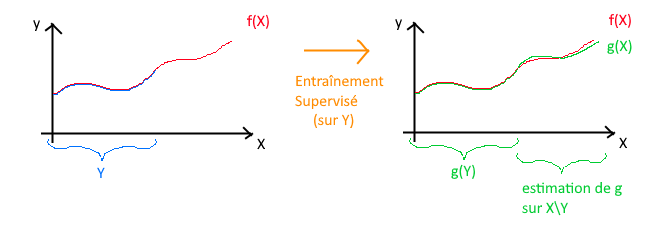
\includegraphics[scale=0.65]{super_schema}
	\end{figure}
\end{frame}

\begin{frame}
	\frametitle{Principe de l'apprentissage supervisée}
	La création du modèle passe par l'optimisation d'une fonction d'objectif, où les paramètres à optimiser sont ceux du modèle.
	Exemple avec une regression linéaire dont le modèle est de la forme :
	\begin{figure}[h]
		\centering
		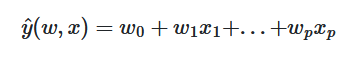
\includegraphics[scale=0.7]{f_lineair}
		\caption{$x$ les données, $w$ les paramètres}
	\end{figure}
	\alert{N.B : refaire la figure (celle-ci est volée du manuel scikit)}
\end{frame}

\begin{frame}
	\frametitle{ElasticNet}
	
	\begin{figure}[b]
		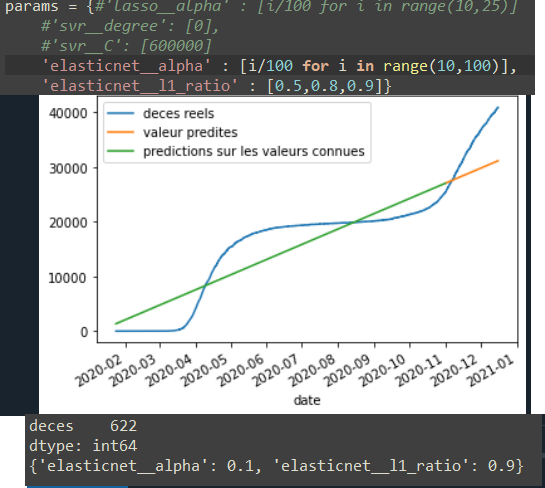
\includegraphics[scale=0.35]{EN}
		\centering
		\caption{résultats peu intéressant dans notre cas..}
	\end{figure}
\end{frame}

\subsection{Optimisation d'hyperparamètres et stratégies}
\subsubsection{Cross-validation}
\begin{frame}
	\frametitle{Recherche du meilleur paramètre}
	Principe de la  "cross-validation" :
	\begin{figure}[b]
		\centering
		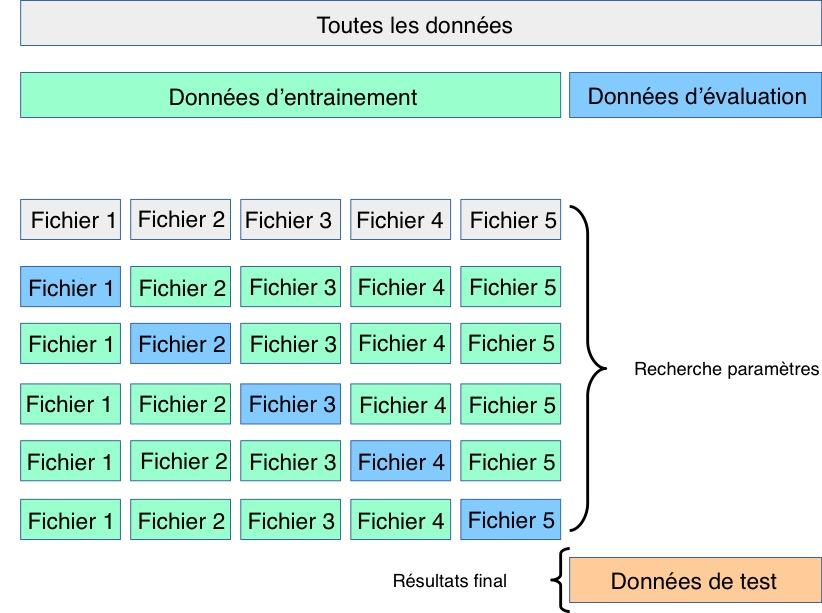
\includegraphics[scale=0.27]{gscv}
	\end{figure}
\end{frame}

\subsection{Résultats avec SVR}
\begin{frame}
	\frametitle{SVR ; premier résultat}
	Approche à l'aide du modèle SVR. 
	
	Noyau 'rbf' $\rightarrow$ ajustement du paramètre C
	\begin{figure}[tc]
		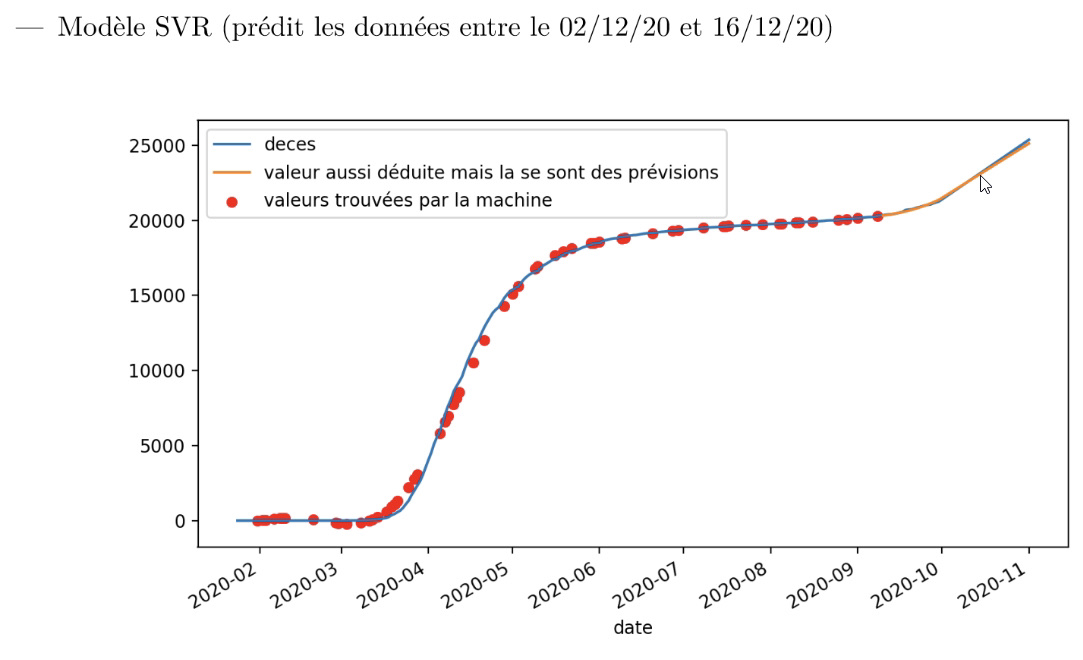
\includegraphics[scale=0.2]{SVR_premierdecoup}
		\centering
		\caption{Premier résultat avec SVR et découpage inadapté}
	\end{figure}
\end{frame}

\subsubsection{Découpages adaptés}
\begin{frame}
	\frametitle{Découpage adapté pour la CV}
		Remise en question de la méthode de découpage
		\begin{figure}[h]
			\centering
			\begin{minipage}{0.5\textwidth}
				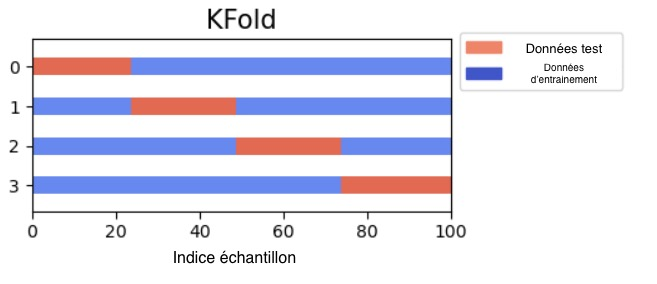
\includegraphics[scale=0.3]{kfold}
			\end{minipage}
			\centering
			\begin{minipage}{0.5\textwidth}
				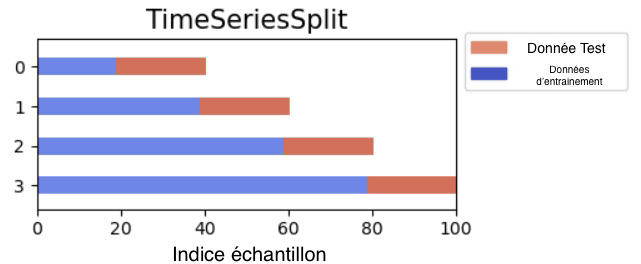
\includegraphics[scale=0.3]{tscv}
			\end{minipage}
		\caption{Comparaison des découpages pour la CV}
		\end{figure}
\end{frame}

\begin{frame}
	\frametitle{SVR}
	\begin{figure}[t]
		\centering
		\begin{minipage}{0.5\textwidth}
			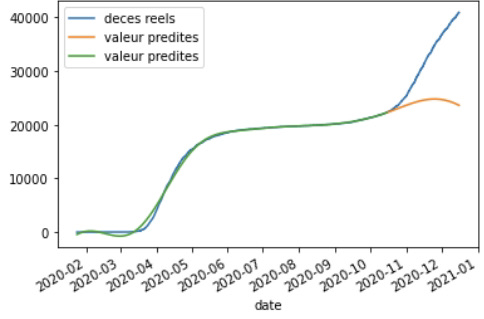
\includegraphics[scale=0.25]{SVR_avant_pt_dinflexion}
		\end{minipage}%
		\begin{minipage}{0.5\textwidth}
			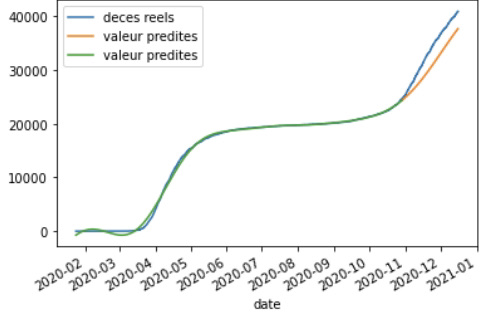
\includegraphics[scale=0.25]{SVR_apres_pt_dinflexion}
		\end{minipage}
	\caption{à gauche la prediction avant le pt d'inflexion, à droite, après.}
	\end{figure}
	$\Rightarrow$ Le modèle n'arrive pas à "suivre" sans le point d'inflexion.
\end{frame}


\section{Approche multivariées}
\subsection{Multiregresseur : 'RegressorChain'}
\begin{frame}
	\frametitle{RegressorChain SVR}
	Multiregresseur RegressorChain\\ Corrélation: Cas confirmé $\rightarrow$ hospitalisé $\rightarrow$ décès 
	
	\begin{figure}[h]
		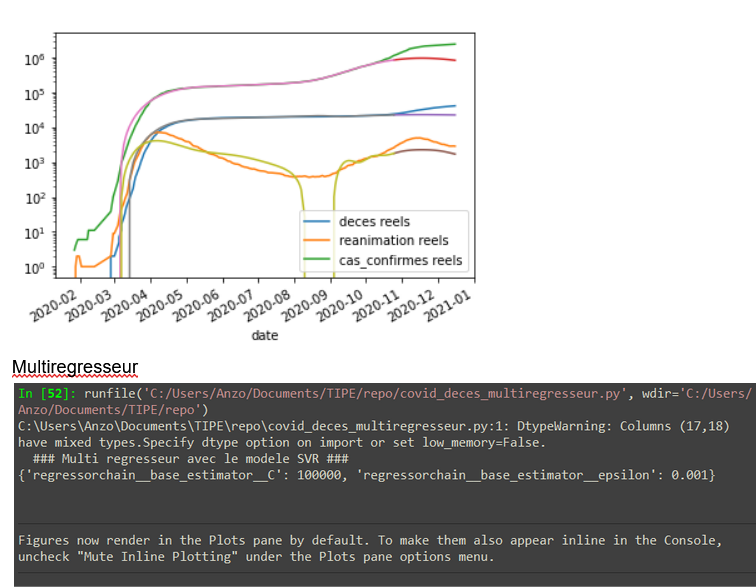
\includegraphics[scale=0.45]{mulitregr_epic_fail}%modifier le fichier
		\caption{résultat avec SVR (insatisfaisant)}
	\end{figure}
\end{frame}

\subsection{Réseau neuronal}
\begin{frame}
	\frametitle{Explications}
	Approche avec des réseau neuronaux
	\begin{figure}[t]
		\centering
		\begin{minipage}{0.5\textwidth}
			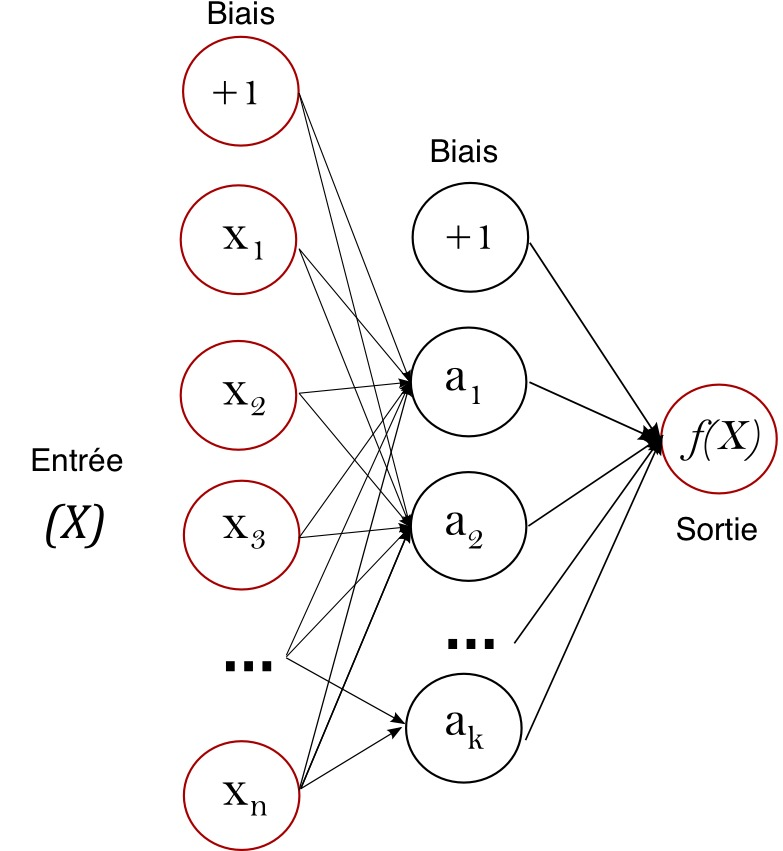
\includegraphics[scale=0.2]{nn_sk}
		\end{minipage}
	\caption{échec du modèle sans la courbe des cas confirmés}
	\end{figure}
\end{frame}

\begin{frame}
	\frametitle{Résultats}
	\begin{figure}[h]
		\centering
		\begin{minipage}{0.5\textwidth}
			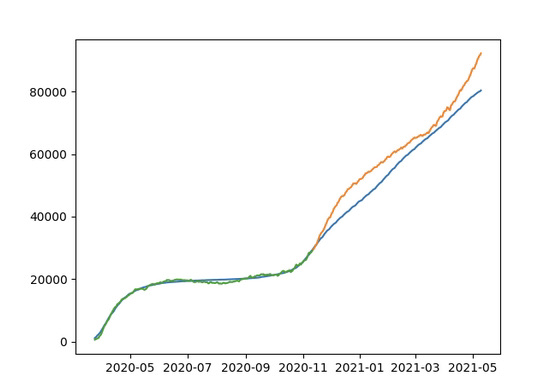
\includegraphics[width=\textwidth]{NN_1}
			\centering
		\end{minipage}
		\begin{minipage}{0.5\textwidth}
			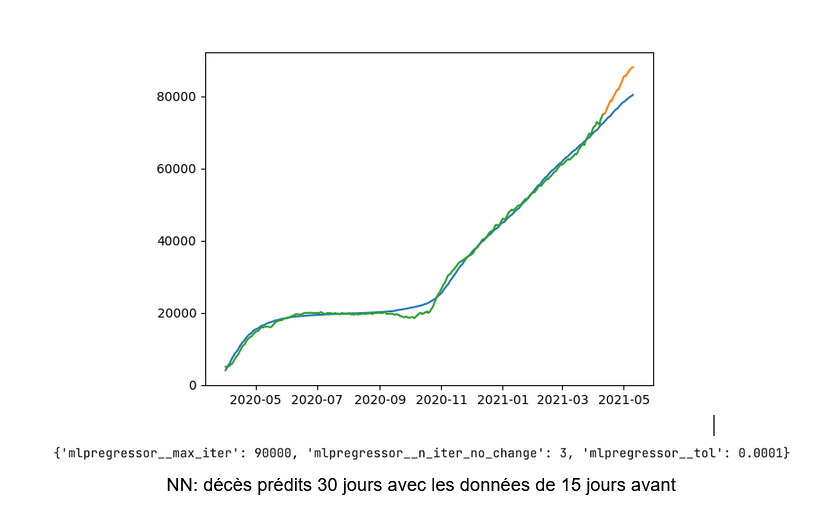
\includegraphics[width=\textwidth]{NN_2}
			\centering
		\end{minipage}
	\caption{échec du modèle sans la courbe des cas confirmés}
	\end{figure}
\end{frame}

\begin{frame}
	\frametitle{Résultats}
	\begin{figure}
		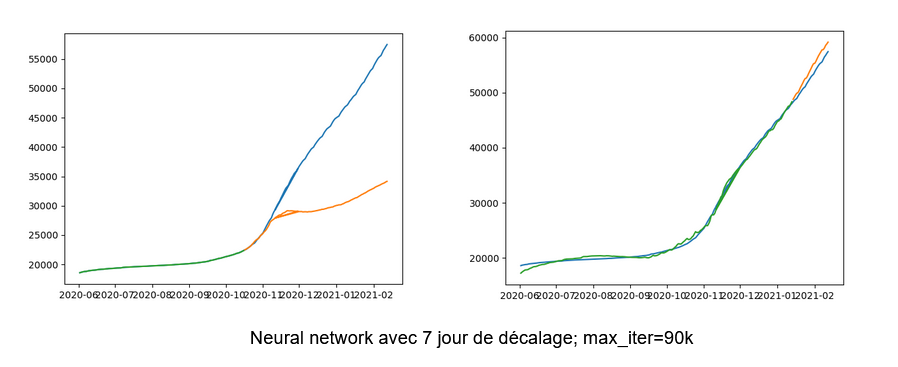
\includegraphics[scale=0.6]{NN_3}
		\caption{échec du modèle sans la courbe des cas confirmés}
	\end{figure}
\end{frame}

\begin{frame}
	\frametitle{Notes}
	\alert{N.B les diapos sont trop verbeux; il faut encore un effort de concision, ou alors elles doivent être expliquées à l'oral}\\
	\alert{N.B sourcer les images}
\end{frame}

\end{document}
